\documentclass{article}
\usepackage[brazil]{babel}
\usepackage[utf8]{inputenc}
\usepackage{graphicx}
\usepackage{indentfirst}


\title{Trabalho 1 de SSC0503 - Introdução à Ciência de Computação II}
\author{Andrey Garcia - 10734290 Gabriel Morão - 7236785 Karina Tiemi - 7978779}
\date{September 2018}


\begin{document}

\maketitle

\section{Introdução}
Neste trabalho serão coletados dados referentes a oito algoritmos de ordenação, sendo eles o Bubble Sort, o Bubble Sort com Sentinela, o Cocktail Sort, O Selection Sort, O Insertion Sort, O Merge Sort, O Heapsort e por fim o Quicksort.
Tais dados são referentes a quantas atribuições e comparações são feitas durante a execução do algoritmo em vetores de tamanhos 100,1000,10000,100000,1000000 em quatro situações diferentes, uma de vetores aleatórios, uma de vetores parcialmente ordenados, uma de vetores quase inversamente ordenadas e por fim uma de vetores com vários valores repetidos.

Foram usados 8 códigos em linguagem C que se encontram nas pastas com o nome dos algoritmos referentes a cada um, também encontra-se o projeto no codeblocks usado em cada um deles(Os códigos contém comandos para o sistema, como o "system("PAUSE")" e "system("CLS")" que podem não ser executados dependedno do sistema operacional utilizado para rodar o algoritmo, sendo assim eles estão na forma de comentario, no entanto foram usados para a coleta dos dados). Para cada tipo de vetor e tamanho o algoritmo foi rodado \textbf{cinco} vezes afim de obter a média do número de comparações e atribuições.

Na seção abaixo encontram-se os dados referentes a cada tipo de vetor coletados para a discução do trabalho seguindo a respectiva ordem: Vetores Aleatórios, Vetores Quase Ordenados, Vetores Quase Inversamente Ordenados e Vetores com Muitos Valores Repetidos.
\section{Dados e Tabelas}
    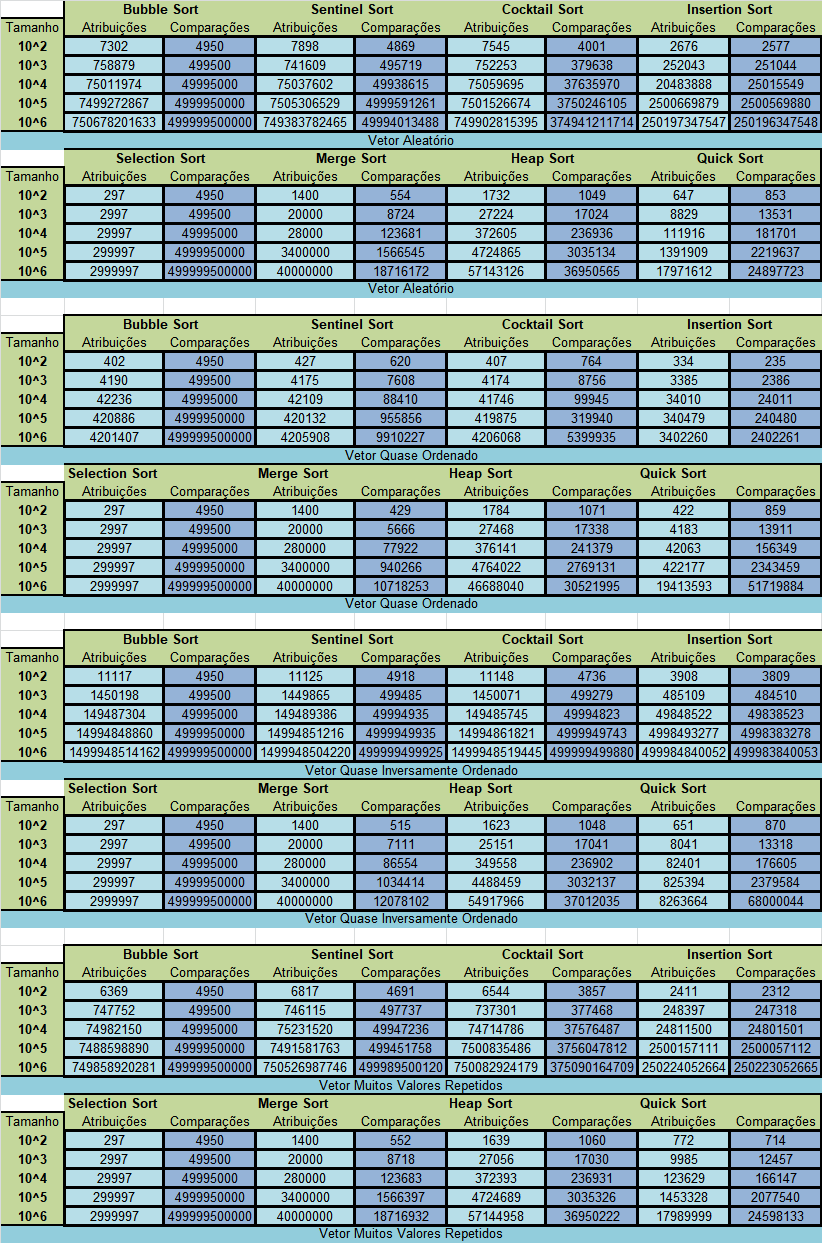
\includegraphics[width=\textwidth,height=\textheight,keepaspectratio=true]{{Images/tabeela}}
\section{Análise dos algoritmos}
Nesta seção serão analisados os dados extraídos de cada algoritmo em cada um dos cenários analisados.
\begin{itemize}
    \item \textbf{Bubble Sort}: Esse algoritmo teve seu melhor desempenho em vetores quase ordenados, e seu pior desempenho deu-se no caso de vetores quase inversamente ordenados. É interessante notar que este algoritmo faz um número fixo de comparações entre elementos do vetor independente se ele e aleatório, quase ordenado, quase inversamente ordenado ou com vários valores repetidos.
    \item \textbf{Bubble Sort com sentinela (Sentinel Sort)}: Esse algoritmo teve seu melhor desempenho em vetores quase ordenados, e seu pior desempenho deu-se no caso de vetores quase inversamente ordenados. Diferentemente de sua implementação sem sentinela, o número de comparações varia dependendo do tipo de vetor usado, consequentemente, ele realiza em média menos operações que sua versão sem sentinela.
    \item \textbf{Bubble Sort com coquetel}:Observa-se que para este algoritmo, o melhor desempenho foi para vetores quase ordenados, enquanto que quase inversamente ordenados apresentou o pior desempenho. De forma análoga, com exceção do quase ordenado que apresentou valores muito próximos para todos os tamanhos, como era de se esperar o tempo decorrido para aumento do tamanho do vetor era notório, característica de sua complexidade. Assim como o algoritmo com sentinela, o número de comparações varia dependendo do tipo de vetor, algumas vezes variando dentro do próprio tipo.
    \item \textbf{Insertion Sort}: Esse algoritmo teve seu melhor desempenho em vetores quase ordenados, vale a pena notar que para esse caso o algoritmo tem o seu desempenho quase 85000 vezes melhor. Já seu pior desempenho deu-se no caso de vetores quase inversamente ordenados.
    \item \textbf{Selection Sort}: Como se era esperado, não há melhor ou pior caso quando se compara os tipos de vetor, pois o modo como o algoritmo funciona apresenta o mesmo valor de comparações e atribuições para todos. Ao comparar os diferentes tamanhos, também como se era esperado, vemos um aumento constante, onde se o tamanho é aumento 10 vezes, o número de atribuições e comparações também é. O tempo decorrido para cada análise também foi como esperado, não havendo muita diferença para tamanhos menores, mas ao chegarmos no maior tamanho o tempo cresce significativamente.
    \item \textbf{Merge Sort}: Esse algoritmo teve seu melhor desempenho em vetores quase ordenados, e seu pior desempenho deu-se no caso de vetores totalmente aleatórios, apesar de as diferenças entre o desempenho em cada caso não ser tão grande. Um fato interessante é que esse algoritmo faz um número fixo de atribuições com elementos do vetor para cada um dos tamanhos das estruturas de dados independentemente de serem valores totalmente aleatórios, quase ordenados, quase inversamente ordenados ou com muitos valores repetidos.
    \item \textbf{Heapsort}: Todos os valores de tempo foram muito próximos para este algoritmo, observando-se que por pouco o pior caso encontrado foi para vetores quase inversamente ordenados enquanto que o melhor caso varia entre os outros 3, dependendo do tamanho, sendo no vetor quase ordenado a apresentação de melhor desempenho. O número de comparações não se manteve constante nem entre tipos de vetores e nem em tamanho. No primeiro observa-se que apesar da variação, os valores médios são muitos próximos, enquanto que no segundo caso observa-se o aumento esperado de acordo com o tamanho do vetor.
    \item \textbf{Quicksort}: Neste algoritmo, para pequenos tamanhos de vetor não se nota diferença significativa de tempo, porém ao nos aproximarmos de tamanhos maiores de vetor, os de tipo vetor aleatório e quase inversamente ordenado saem na frente, onde o segundo é infimamente melhor até o caso de maior vetor, onde apresentou pior desempenho que todos os outros tipos. Por diferença ínfima também, observa-se que o pior desempenho seria para o vetor quase ordenado.
    OBS : Para a implementação desse algoritmo foi usado um pivô com um número aleatório selecionado a cada chamada recursiva do algoritmo.
\end{itemize}
\section{Comparações entre os algoritmos}
Nesta seção serão comparados os algoritmos, em relação a número de comparações e de atribuições em cada caso.


\begin{enumerate}
    \item \textbf{Vetores Aleatorios.}
    
     Para vetores aleatórios o algoritmo que teve melhor desempenho em relação as comparações (para todos os tamanhos) foi o Merge Sort, seguido pelo Quicksort e pelo Heapsort, os outros algoritmos fazem muito mais comparações que estes seguindo a ordem, do que faz menos comparações para o que faz mais: Insertion Sort, Cocktail Sort, Bubble Sort com Sentinela, Bubble Sort e Selection Sort empatados como os que fazem mais comparações. 
   
     Já em relação ao número de atribuições a situação é diferente, o algoritmo que realiza menos trocas é o Selection Sort para todos os tamanhos de vetor. Depois dele vêm o Quicksort, o Merge Sort e o Heapsort, por fim temos o Insertion Sort, o Cocktail Sort, o Bubble Sort com Sentinela e por fim o Bubble Sort.
     
     Os resultados estão de acordo com o esperado pela complexidade dos algotirmos. O Merge Sort e o Heap Sort possuem complexidade O(nlogn) enquanto o Quick Sort pode ser também do mesmo no caso médio mas O(n²) no pior caso. Todos os outros algoritmos estudados apresentam complexidade O(n²) para comparações, o que explica seu pior desempenho neste quesito. Para as atribuições (ou trocas), o Selection Sort apresenta complexidade O(n), seguido por Quick, Merge e Heap Sort com complexidades O(nlogn) e os últimos, O(n²).
     
    
    \item \textbf{Vetores Quase Ordenados.}
    Para vetores quase ordenados o algoritmo que obteve o melhor desempenho em relação ao número de comparações foi disparadamente o Insertion Sort para todos os tamanhos de vetor, seguido dele vêm o Cocktail Sort, e o Bubble Sort com Sentinela para tamanhos maiores que 100000 e  o Merge Sort para tamanhos menores que 100000, em seguida, para tamanhos até 100000, o Quicksort tem uma ligeira vantagem em relação ao Heapsort que e perdida no caso do tamanho 1000000. Por fim vêm o Bubble e o Selection Sort na última colocação.
    
	Em relação as atribuições nota-se também uma vantagem do Selection Sort em relação aos outros métodos que não e tão grande quanto para vetores totalmente aleatórios, mas ainda assim o método se dá melhor nessa ocasião, seguido de perto pelo Insertion Sort depois pelas variações do Bubble Sort. Já o algoritmo que teve o pior desempenho em relação as atribuições foi o Heapsort.
	
	Neste caso os resultados são explicados principalmente pelo funcionamento do código e em como são feitas as comparações. O fato do vetor estar quase ordenado indica que poucas atribuições deverão ser realizadas e assim o vetor se ordena mais rapidamente, não necessitando de mais comparações. Os outros algoritmos funcionam de forma diferente, separando o vetor e/ou o bagunçando antes/durante a ordenação, o que acaba a atrasando a ordenação e necessitando de mais comparações.
	
	\item \textbf{Vetores Quase Inversamente Ordenados.}
	Para esse tipo de dado o algoritmo que obteve o melhor desempenho em relação ao número de comparações foi o Merge Sort seguido do Quicksort e pelo Heapsort, isso Para vetores de até 100000 posições, a partir disso esses dois ultimos algoritmos invertem-se em relação a seu desempenho. Por fim temos o Insertion Sort, Cocktail Sort, Sentinel Sort e por fim Bubble Sort e Selection Sort como os piores para esse caso.
	
	Já em relação ao número de atribuições o Selection Sort continua sendo quem realiza menos, seguido Quicksort, Mergesort e Heapsort. Com um desempenho mediano para esse quesito temos o Sentinel Sort, o Bubble Sort e o Cocktail Sort e por fim o Insertion Sort tem o pior desempenho nesse caso.
	
	Assim como no caso dos Vetores Quase Ordenados, o modo de operação influencia muito. Novamente como está quase ordenado, o Selection Sort precisa de menos trocas, mas mais que anteriormente pois agora deve "desinveter" o vetor, mas como suas comparações se iniciam no começo do vetor, seu número é grande. Os outros algoritmos quadraticos vão trabalhar de forma semelhante ao Vetor Quase Ordenado, porém pela inversão apresentada do vetor, o número de comparações e trocas é grande os limitando muito. Como o Heap, Quick e Merge não se importam com a ordenação inicial, não são afetados pela inversão do vetor e apresentam resultados proximos dos anteriores, ficando atrás do Selection e a frente dos outros.
	
	\item \textbf{Vetores Vetor Muitos Valores Repetidos}
	Neste caso, em relação ao número de comparações foi o Merge Sort, seguido do Quicksort e do Heapsort, com valores intermediários, temos o Insertion Sort e o Cocktail Sort, ja os que ocupam os piores lugares nesssa comparação são o Sentinel Sort, e o Selection e Bubble Sort empatados na ultima posição.
	
	Para as atribuições quem se da melhor como nos casos anteriores ainda é o Selection Sort seguido do Quicksort, do Merge Sort e do Heapsort, seguindo deles temos o Insertion Sort, o Cocktail Sort, o Sentinel Sort e o Bubble Sort(variando entre esses três ultimos qual é o melhor, para vetores até 10000 posições o Cocktail Sort faz menos comparações, a partir dai quem faz menos e o Bubble Sort, seguido do Sentinel Sort e por fim do próprio Cocktail Sort).
	
	Os métodos de ordenação quadráticos não levam tanto em consideração os valores repetidos, realizando comparações desnecessárias diversas vezes até que o vetor esteja ordenado. Por isso, os algoritmos não quadráticos saem em vantagem neste quesito. Para as atribuições o mesmo pensamento se aplica, porém o Selection Sort continua apresentando complexidade O(n), selecionando o menor e o endereçando a posição inicial para cada varredura,realizando assim um menor número de trocas. 
	
\end{enumerate}
\section{Conclusões}

   Aqui será dito, avaliando \textbf{apenas} o número de comparações e atribuições (dado isso, coisas como tempo de execução, estabilidade do método, quantidade de espaço extra ou qualquer outra característica relacionada aos algoritmos serão ignoradas para tal conclusão), qual(quais) algoritmos usar para cada tipo de vetor e qual tamanho. \par 
    
    Para todos os tipos de vetores e tamanhos, se o processo de realizar atribuições for algo muito custoso o Selection Sort e a melhor opção para se usar independentemente do tipo de vetor, pois faz o mesmo número de atribuições, que consegue ser menor que os outros, em todas as situações.
    
    Caso contrário para vetores aleatórios os métodos que se saíram melhor, levando em conta o número de comparações e atribuições foram o Merge Sort o Quicksort. Já para vetores quase ordenados, quem se sai melhor é o Insertion Sort seguido pelas variações do Bubble Sort. Já para vetores quase inversamente ordenados de até 100000 posições o Quicksort é o mais indicado, depois disso a situação muda e quem tem o melhor desempenho é o Merge Sort. Por fim para vetores com muitos valores repetidos o Quicksort se destaca como quem faz menos operações.

\end{document}
